%!TEX root = ../main.tex
\noindent \textbf{\large APPENDIX}
\vspace{1em}  


%%% database knobs (impactful; secondary)
\noindent \textbf{\large A DATABASE KNOBS}
\label{sec: databaseKnobs}

Take PostgreSQL as an Instance. It exposes 247 knobs for users to tune the performance, in which 66 are tunable. As shown in Table~\ref{tbl:knob}, there are 12 impactful knobs, which can take direct effects in some scenarios and are commonly used by the DBA; other 55 extended knobs can take indirect effect to the database performance, usually in long term, such as the knobs of checkpoints, autovacuum and deadlocks.

% Please add the following required packages to your document preamble:
% \usepackage[normalem]{ulem}
% \useunder{\uline}{\ul}{}
% Please add the following required packages to your document preamble:
% \usepackage[normalem]{ulem}
% \useunder{\uline}{\ul}{}
\begin{table*}[hb]
\centering
\vspace{-1.5em}
\caption{Tunable knobs in PostgreSQL. $"*$\_table\_age$"$ denotes vacuum\_multixact\_freeze\_table\_age.}
\label{tbl:knob}
{
\begin{tabular}{lllll}\hline
\textbf{\textit{Impactful Knob}}  & \multicolumn{3}{c}{\textbf{\textit{Extended Knob}}}                                                                                                    \\\hline
effective\_io\_concurrency     & deadlock\_timeout         & checkpoint\_warning            & pre\_auth\_delay                \\
statement\_timeout             & bgwriter\_delay           & geqo\_threshold                & max\_wal\_size                  \\
effective\_cache\_size         & bgwriter\_lru\_maxpages   & geqo\_selection\_bias          & min\_wal\_size                  \\
work\_mem                      & geqo\_pool\_size          & geqo\_effort                   & autovacuum\_analyze\_threshold  \\
commit\_delay                  & checkpoint\_timeout       & geqo\_generations              & autovacuum\_naptime             \\
temp\_buffers                  & maintenance\_work\_mem    & log\_autovacuum\_min\_duration & autovacuum\_vacuum\_cost\_delay \\
max\_stack\_depth              & temp\_file\_limit         & log\_file\_mode                & autovacuum\_vacuum\_cost\_limit \\
from\_collapse\_limit          & tcp\_keepalives\_count    & log\_min\_duration\_statement  & autovacuum\_vacuum\_threshold   \\
commit\_siblings               & tcp\_keepalives\_idle     & log\_rotation\_age             & autovacuum\_work\_mem           \\
join\_collapse\_limit          & tcp\_keepalives\_interval & log\_rotation\_size            & vacuum\_cost\_delay             \\
max\_standby\_archive\_delay   & archive\_timeout          & log\_temp\_files               & vacuum\_cost\_limit             \\
max\_standby\_streaming\_delay & authentication\_timeout   & post\_auth\_delay              & vacuum\_cost\_page\_dirty       \\
                               & gin\_fuzzy\_search\_limit & gin\_fuzzy\_search\_limit      & vacuum\_cost\_page\_hit         \\
                               & vacuum\_cost\_page\_miss  &        vacuum\_freeze\_min\_age      &   vacuum\_freeze\_table\_age \\
                               & vacuum\_multixact\_freeze\_min\_age  & $*$\_table\_age &   wal\_keep\_segments \\
                               & wal\_receiver\_status\_interval  & wal\_receiver\_timeout &   wal\_retrieve\_retry\_interval \\
                               & wal\_sender\_timeout  & wal\_writer\_delay & gin\_fuzzy\_search\_limit \\
                               
                               & gin\_pending\_list\_limit  & allow\_system\_table\_mods & default\_statistics\_target \\                               
            &extra\_float\_digits & & \\\hline

\end{tabular}
}
\end{table*}


%%% database state
\vspace{1.5em}
\noindent \textbf{\large B DATABASE METRICS}
\label{sec: databaseMetrics}

This section lists all the database metrics used as the outer metrics information in the DS-DDPG model. as shown in Table~\ref{tbl:state}, they are classified into two types: meta parameters and cumulative statistics. Meta parameter indicates important untunable knobs in the database, which can reflect some important configurations of the database, such as the size of shared buffer. Cumulative statistics indicate important database activities, such as the total number of read blocks and backends. We use the cumulative statistics to reflect the database burden.

\begin{table*}[ht]
\centering
\caption{Metrics of database state in PostgreSQL}
\label{tbl:state}
\vspace{0.5em}
{
\begin{tabular}{llllll}\hline
\multirow{2}{*}{\textbf{\textit{Meta Parameter}}} & & \multicolumn{4}{c}{\textbf{\textit{Cumulative Statistics}}}             \\

                                  & $\ \ \ \ \ \ \ \ $  & \textbf{\textit{DB-wide}} &  $\ \ \ \ \ \ \ \ $  & \multicolumn{2}{c}{\textbf{\textit{User level}}}  \\\hline
               shared\_buffers      &     & heap\_blks\_read  &  & numbackends    & tup\_returned    \\
               max\_connections     &        & heap\_blks\_hit  & & xact\_commit   & tup\_fetched     \\
               wal\_buffers      &      & idx\_blks\_read &  & xact\_rollback & tup\_inserted    \\
              max\_worker\_processes   &     & idx\_blks\_hit   & & blks\_read     & tup\_updated     \\
          max\_prepared\_transactions    &        & toast\_blks\_read & & blks\_hit      & tup\_deleted     \\
 max\_files\_per\_process    &          & toast\_blks\_hit &  & conflicts      & deadlocks        \\
                              &       & tidx\_blks\_read &  & temp\_files    & blk\_read\_time  \\
                               &      & tidx\_blks\_hit   & & temp\_bytes    & blk\_write\_time \\\hline
\end{tabular}
}
\end{table*}


%%% Accuracy of tuning in query level
\vspace{1.5em}
\noindent \textbf{\large C Evaluation on Accuracy}
\label{sec: accuracy}

To evaluate how well \oursys performs for different queries, or the accuracy of tuning in query level, here we also conduct experiments on PostgreSQL with physical environment (128G RAM, 5T Disk). For 113 queries in JOB benchmark, we randomly choose 64 queries, and evaluate the performance of these queries with DBA, CDBTune and \oursys respectively. In Fig~\ref{fig:accuracy}, We sort the points by the  percent of latency reduction with \oursys. We can find that, the performance of \oursys for different queries is very stable and the average value is better than the other two methods. The performance of CDBTune is relatively steady, around 60$\%$ reduction in average. While it may be hard for DBA to tune in query-level, he has trouble in accurately tuning for different queries.

%%% Network arch
\vspace{2.5em}
\noindent \textbf{\large D Network architecture}
\label{sec:network}

In this section, we demonstrate the basic architectures of two networks, the Actor and Critic in the DS-DDPG model. They are both fully connected neural networks of six layers. We show the types of layers and the detailed activation functions in each layer in Table~\ref{tbl:actor} and Table~\ref{tbl:critic}. The Actor accepts the observation features and outputs the knob configurations. And the Critic accepts (observation, action) and outputs a score (Q-value). They are designed based on the concepts we have talked in Section~\ref{sec:tunner_training_ac}.




\begin{table}[H]
\caption{The network architecture of the Actor in DS-DDPG. \texttt{S'} denotes the predicted outer metrics, \texttt{A} denotes the output actions and \texttt{V} denotes the feature vector of the workload.}
\centering  
%\subtable{  
	\begin{tabular}{c|c|c|c}\hline
	\multirow{2}{*}{$\textbf{Level}$} & \multicolumn{3}{c}{$\textbf{Actor\ Network}$} \\
	& \multicolumn{1}{c|}{$\textbf{Layer}$} & $\textbf{Activation\ Function}$ & $\textbf{Scale}$\\ \hline
	1 & Input & None & $|$ S' $|$ \\
	2 & Dense & ReLU & $|$ S' $|$ $\times$ 2\\
	3 & BatchNormal & None & $|$ S' $|$ $\times$ 2\\
	4 & Dense & ReLU & $|$ S' $|$ / 2\\
	5 & Dropout & None & $|$ S' $|$ / 2\\
	6 & Dense & TargetRange & $|$ A $|$\\\hline
	\end{tabular} 
%}    
\label{tbl:actor}    
\end{table} 

\begin{table}[H]
\caption{The network architecture of the Critic in DS-DDPG. \texttt{M} denotes max($|$\texttt{S'}$|$, $|$\texttt{A}$|$).}
\centering  
	\begin{tabular}{c|c|c|c}\hline
	\multirow{2}{*}{$\textbf{Level}$} & \multicolumn{3}{c}{$\textbf{Critic\ Network}$} \\
	& \multicolumn{1}{c|}{$\textbf{Layer}$} & $\textbf{Activation\ Function}$ & $\textbf{Scale}$\\ \hline
	
	1 & Dense & ReLU & $\ \ $M + M\\
	2 & Dense & None & $\ $M\\
	3 & Dense & tanh & $\ $M / 2\\	
	4 & Dropout & None & $\ $M / 2\\
	5 & BatchNormal & None & $\ $M / 2\\
	6 & Dense & None & $\ $1\\\hline
  \end{tabular}

\label{tbl:critic}    
\end{table} 


\begin{figure}[htb]
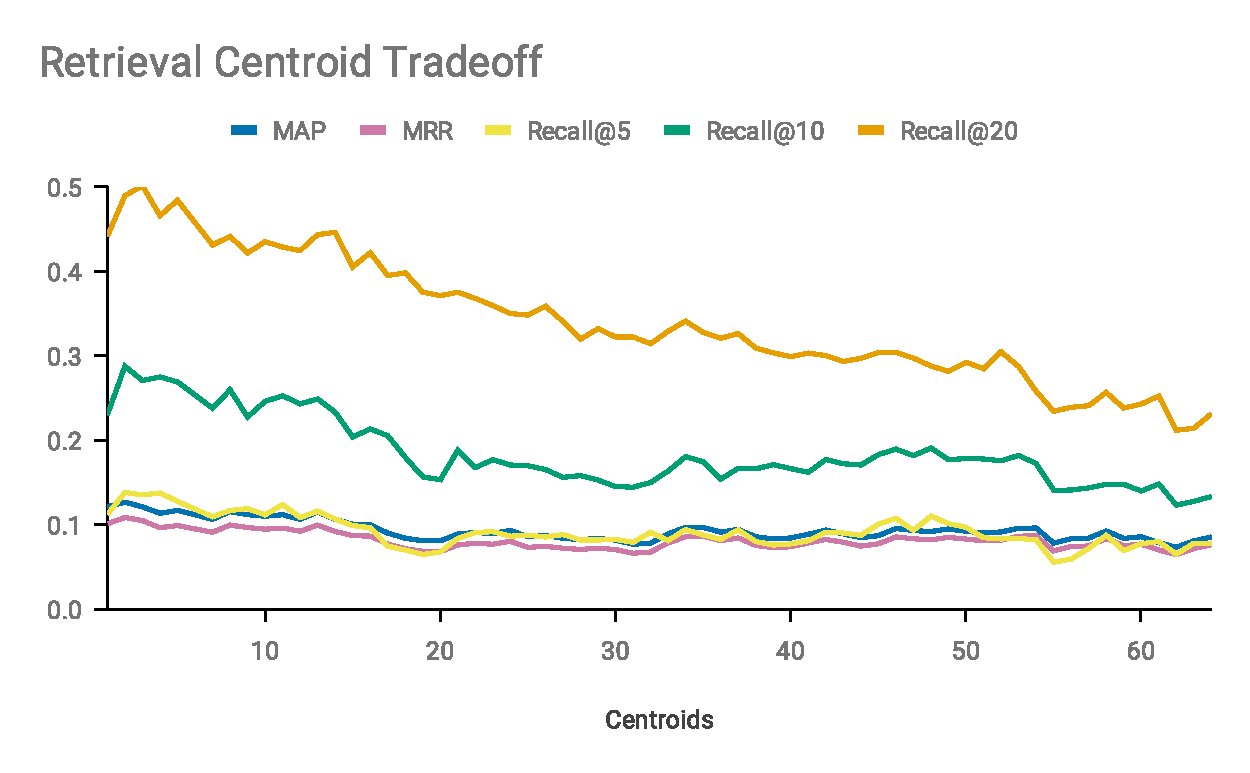
\includegraphics[width=0.48\textwidth, height=0.40\textwidth]{tuning_figs/accuracy.eps}
\vspace{-2em}
\caption{The accuracy of tuning in query level, for DBA, CDBTune and \oursys .}
\label{fig:accuracy}
\vspace{-0.5em}
\end{figure} 


%%% Configuration Instance
\vspace{1.0 em}
\noindent \textbf{\large E Configuration Instance}
\label{sec:config}

In this section we show the configuration instances for the TPC-H benchmark running on PostgreSQL in Tables~\ref{tbl:knobDefault},~\ref{tbl:knobDBA} and~\ref{tbl:knobQTune}. For the configurations generated by QTune, out of the 64 tunable knobs, here we only display 20 knobs most frequently adjusted by the Tuner. Since most queries in TPC-H are CPU-intensive,  QTune has tuned the values of max\_connections and join\_collapse\_limit higher.

\begin{table}[H]
\caption{A configuration instance of DBA.}
\centering  
%\subtable{  
	\begin{tabular}{lll}\hline
	$\textbf{Knob}$ & & \textbf{Value} \\\hline
	effective\_cache\_size & $\ \ \ $ & 8192 \\
	work\_mem & $\ \ \ $ & 256 MB \\
	commit\_delay & $\ \ \ $ & 0 \\
	max\_stack\_depth & $\ \ \ $ & 2048 \\
	deadlock\_timeout & $\ \ \ $ & 2000 \\
	from\_collapse\_limit & $\ \ \ $ & 8 \\
	lock\_timeout & $\ \ \ $ & 20 min \\
	join\_collapse\_limit & $\ \ \ $ & 4 \\	
	log\_file\_mode & $\ \ \ $ & 384 \\
	checkpoint\_completion\_target & $\ \ \ $ & 0.5 \\\hline

	\end{tabular} 
%}    
\label{tbl:knobQTune}    
\end{table} 

\begin{table}[H]
\caption{A configuration instance of \oursys.}
\centering  
%\subtable{  
	\begin{tabular}{lll}\hline
	$\textbf{Knob}$ & & \textbf{Value} \\\hline
	effective\_cache\_size & $\ \ \ $ & 8192 \\
	work\_mem & $\ \ \ $ & 6 GB \\
	commit\_delay & $\ \ \ $ & 10 \\
	max\_stack\_depth & $\ \ \ $ & 2048 \\
	deadlock\_timeout & $\ \ \ $ & 100 \\
	from\_collapse\_limit & $\ \ \ $ & 8 \\
	lock\_timeout & $\ \ \ $ & 1 min \\
	join\_collapse\_limit & $\ \ \ $ & 4 \\	
	log\_file\_mode & $\ \ \ $ & 384 \\
	checkpoint\_completion\_target & $\ \ \ $ & 10 \\
	bulk\_write\_ring\_size  & $\ \ \ $ & 16 MB \\ %%
	default\_statistics\_target & $\ \ \ $ & -2 \\
	maintenance\_work\_mem & $\ \ \ $ & 256 MB \\
	max\_active\_statements & $\ \ \ $ & 1000 \\
	max\_connections & $\ \ \ $ & 1000 \\
	max\_prepared\_transactions & $\ \ \ $ & 1000 \\
	statement\_timeout & $\ \ \ $ & 6000000 \\
	wal\_buffers & $\ \ \ $ & 512 \\
	wal\_keep\_segments & $\ \ \ $ & 256 \\
	walsender\_max\_send\_size & $\ \ \ $ & 2048 \\\hline

	\end{tabular} 
%}    
\label{tbl:knobDBA}    
\end{table} 

\vspace{-1em}
\begin{table}[H]
\caption{The default configuration.}
\centering  
%\subtable{  
	\begin{tabular}{lll}\hline
	$\textbf{Knob}$ & & \textbf{Value} \\\hline
	effective\_cache\_size & $\ \ \ $ & 256 \\
	work\_mem & $\ \ \ $ & 4096 KB \\
	commit\_delay & $\ \ \ $ & 0 \\
	max\_stack\_depth & $\ \ \ $ & 100 \\
	deadlock\_timeout & $\ \ \ $ & 1000 \\
	from\_collapse\_limit & $\ \ \ $ & 8 \\
	lock\_timeout & $\ \ \ $ & 0 \\
	join\_collapse\_limit & $\ \ \ $ & 8 \\	
	log\_file\_mode & $\ \ \ $ & 600 \\
	checkpoint\_completion\_target & $\ \ \ $ & 0.5 \\
	bulk\_write\_ring\_size  & $\ \ \ $ & 256 KB \\ %%
	default\_statistics\_target & $\ \ \ $ & 100 \\
	maintenance\_work\_mem & $\ \ \ $ & 128 MB \\
	max\_active\_statements & $\ \ \ $ & 6 \\
	max\_connections & $\ \ \ $ & 8 \\
	max\_prepared\_transactions & $\ \ \ $ & 0 \\
	statement\_timeout & $\ \ \ $ & 0 \\
	wal\_buffers & $\ \ \ $ & -1 \\
	wal\_keep\_segments & $\ \ \ $ & 0 \\
	walsender\_max\_send\_size & $\ \ \ $ & 0 \\
	shared\_buffers & $\ \ \ $ & 500 MB \\
	enable\_nestloop & $\ \ \ $ & off \\\hline
	\end{tabular} 
%}    
\label{tbl:knobDefault}    
\end{table} 

